\documentclass[a4paper,12pt]{article}
\usepackage[bahasa]{babel}
\usepackage{graphicx}
\usepackage{multirow}
\usepackage{enumitem}
\usepackage{listings}
\usepackage{adjustbox}
\graphicspath{ {./img/} }
\begin{document}
\title{Laporan Praktikum Statistika Pertemuan 14}
\author{Aldzikri Dwijayanto Prathama 
	\\195410189}
\makeatletter
\begin{titlepage}
	\begin{center}
		{\huge \bfseries \@title }\\[14ex]
		
\includegraphics[scale=.8]{logo}\\[4ex]
		{\large \@author}\\[20ex]
		{\large \bfseries {SEKOLAH TINGGI MANAJEMEN INFORMATIKA DAN KOMPUTER
				AKAKOM YOGYAKARTA}}
	\end{center}


\end{titlepage}
\makeatother
\newpage
\tableofcontents
\newpage
\section{Tujuan}
\begin{enumerate}
    \item Praktikan mampu melakukan analisis data menggunakan uji rata-rata dua populasi independen.
    \item Praktikan mampu melakukan analisis data menggunakan uji rata-rata dua populasi dependen.
\end{enumerate}

\section{Dasar Teori}
\subsection{Uji Hipotesis Mean 2 Populasi Independen (Uji Independen sample t test)}
Uji rata-rata 2 sampel independen (bebas) adalah metode yang digunakan untuk menguji kesamaan rata-rata dari 2 populasi yang bersifat independen. Independen maksudnya adalah bahwa populasi
yang satu tidak dipengaruhi atau tidak berhubungan dengan populasi yang lain. Asumsi yang harus dipenuhi adalah data berdistribusi normal dan variansi kedua populasi sama.\\
Langkah-langkah uji hipotesis :\\
\begin{enumerate}
    \item Hipotesis
        \begin{enumerate}[label = \alph*.]
            \item $H_{0} : \mu_{1} = \mu_{0}$ (uji dua sisi)\\
                $H_{1} : \mu_{1} \neq \mu_{0}$

            \item $H_{0} : \mu_{1} \leq \mu_{0}$ (uji sisi kanan)\\
                $H_{1} : \mu_{1} > \mu_{0}$

            \item $H_{0} : \mu_{1} \geq \mu_{0}$ (uji sisi kiri)\\
                $H_{1} : \mu_{1} < \mu_{0}$

        \end{enumerate}

    \item Tingkat signifikansi $\alpha = 5\%$

    \item Statistik penguji,p\_value

    \item Daerah kritis\\
        $H_{0}$ ditolak jika p\_value $< \alpha$
        
    \item Kesimpulan\\
Syntak dalam R untuk melakukan uji berpasangan data independen adalah\\
\texttt{t.test(X1, X2, alternative=c("two sided"), paired=F, var.equal=T, conf.level=0.95) \#utk uji dua sisi}\\
    \texttt{t.test(X1, X2, alternative=c("greather"),  paired=F, var.equal=T, conf.level=0.95) \#utk uji satu sisi kanan}\\
    \texttt{t.test(X1, X2, alternative=c("less"),  paired=F, var.equal=T, conf.level=0.95) \#utk uji satu sisi kiri}\\
\end{enumerate}

\subsection{Uji Hipotesis Mean 2 Populasi Dependen (Uji Paired t test)}
Uji hipotesis rata-rata 2 populasi dependen juga sering dinamakan uji rata-rata 2 sampel berpasangan atau paired sample t test. Dalam uji ini, suatu populasi diamati/ diberi perlakuan 2 kali,
sehingga dihasilkan pasangan-pasangan data untuk masing-masing anggota populasi. Rata-rata selisih pengamatan pertama dan ke dua dinamakan $\mu D$. 
Misalkan dari suatu populasi diambil sampel sebanyak n, kemudian sampel tersebut diamati dan menghasilkan data X1, X2, ..., Xn. Selanjutnya diamati untuk yang ke dua kalinya dan menghasilkan
data Y1, Y2, ..., Yn. Dengan demikian dari sampel pertama diperoleh data (X1, Y1), dari sampel ke dua diperoleh (X2, Y2), dan seterusnya sampai sampel ke-n diperoleh (Xn, Yn). Rata-rata
selisih pengamatan pertama dan ke dua pada sampel dinamakan $D$ dan standar deviasinya dinamakan sD.
Berikut uji hipotesis untuk rata-rata 2 populasi dependen.:

\begin{enumerate}
    \item Hipotesis
        \begin{enumerate}[label = \alph*.]
            \item $H_{0} : \mu_{D} = \mu_{0}$ (uji dua sisi)\\
                $H_{1} : \mu_{D} \neq \mu_{0}$

            \item $H_{0} : \mu_{D} \leq \mu_{0}$ (uji sisi kanan)\\
                $H_{1} : \mu_{D} > \mu_{0}$

            \item $H_{0} : \mu_{D} \geq \mu_{0}$ (uji sisi kiri)\\
                $H_{1} : \mu_{D} < \mu_{0}$

        \end{enumerate}

    \item Diambil tingkat signifikansi $\alpha$

    \item Statistik penguji,p\_value

    \item Daerah kritis\\
        $H_{0}$ ditolak jika p\_value $< \alpha$ (untuk semua uji)
        
    \item Kesimpulan\\
Syntak dalam R untuk melakukan uji berpasangan data berpasangan adalah\\
\texttt {t.test(X1, X2, alternative=c("two sided"), paired=T, var.equal=T, conf.level=0.95) \#utk uji dua sisi}
\texttt {t.test(X1, X2, alternative=c("greather"),  paired=T, var.equal=T, conf.level=0.95) \#utk uji satu sisi kanan}
\texttt {t.test(X1, X2, alternative=c("less"),  paired=T, var.equal=T, conf.level=0.95) \#utk uji satu sisi kiri}
\end{enumerate}

\section{Pembahasan}
\subsection{Praktik}
\subsubsection{Uji Hipotesis Mean 2 Populasi Independen (Uji Independen sample t test) }
\paragraph* {}
Dipunyai data tentang tinggi siswa kelas 1, diambil sampel 10 siswa dan 10 siswi. Dengan anggapan data diambil dari populasi normal,ujilah apakah bisa dikatakan tinggi siswa dan siswi kelas 1
tersebut sama?
\begin{table}[!ht]
    \centering
\begin{tabular}{|c|c|}
\hline
Siswa & Siswi \\ \hline
120   & 115   \\ \hline
122   & 120   \\ \hline
120   & 118   \\ \hline
138   & 130   \\ \hline
130   & 135   \\ \hline
128   & 126   \\ \hline
132   & 127   \\ \hline
125   & 126   \\ \hline
127   & 125   \\ \hline
130   & 129   \\ \hline
\end{tabular}
\end{table}
\paragraph{Jawab\\}
Pada praktik ini dilakukan uji independen t test\\
Dari soal di atas diketahui:
\begin{enumerate}[label = \alph*.]
    \item Hipotesis \\
        $H_{0} : \mu_{1} = \mu_{0}$ (rata-rata tinggi siswa dan siswi kelas 1 sama)\\
        $H_{1} : \mu_{1} \neq \mu_{0}$(rata-rata tinggi siswa dan siswi kelas 1 tidak sama)
    \item Tingkat signifikansi $\alpha = 5\%$
    \item Statistik uji p\_value
\end{enumerate}
Untuk menguji independen t test berdasarkan soal di atas, masukkan terlebih dahulu data dari tabel, kolom siswa dimasukkan ke dalam variabel dataSiswa, sedangkan kolom siswi dimasukkan ke 
dalam variabel dataSiswi.\\
\begin{center}
    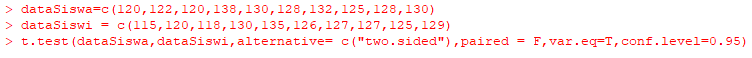
\includegraphics[width = \linewidth]{img1.png}
\end{center}
Setelah itu masukkan variabel ke dalam perintah t.test\\
\texttt{t.test(dataSiswa,dataSiswi,alternative=c("two sided"), paired=F, var.equal=T, conf.level=0.95)}
\begin{center}
    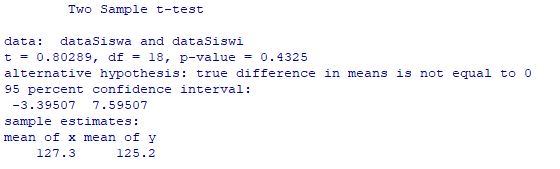
\includegraphics[width = \linewidth]{img2.png}
\end{center}
Dari output diatas diketahui bahwa $H_{0}$ diterima karena $p\_value = 0.4325 > \alpha = 0.05$

\subsubsection{Uji Hipotesis Mean 2 Populasi Dependen (Uji Paired t test)}
\paragraph{}
Bagian akademik ingin melakukan survei terhadap metode  pembelajaran yang baru. Apakah dengan menggunakan metode pembelajaran yang baru memberi dampak kenaikan terhadap IPK mahasiswa penerima.
Nilai $\alpha = 5\%$ (0.05). Dengan data berikut :
\begin{table}[!ht]
    \centering 
\begin{tabular}{|c|c|}
\hline
Sebelum & Sesudah \\ \hline
3.7     & 3.6     \\ \hline
3.6     & 3.7     \\ \hline
3.8     & 3.7     \\ \hline
3.7     & 3.6     \\ \hline
3.9     & 3.6     \\ \hline
3.8     & 3.4     \\ \hline
3.6     & 3.5     \\ \hline
3.9     & 3.5     \\ \hline
\end{tabular}
\end{table}
\paragraph{Jawab\\}
Praktik selanjutnya adalah melakukan uji rata-rata berpasangan\\
Dari soal di atas diketahui:
\begin{enumerate}[label = \alph*.]
    \item hipotesis\\
        $H_{0} : \mu_{sebelum} \geq \mu_{sesudah}$ (rata-rata IPK mahasiswa sebelum menerima metode pembelajaran baru  lebih besar atau sama dengan rata-rata IPK mahasiswa setelah menerima
        metode pembelajaran baru)
        $H_{1} : \mu_{sebelum} < \mu_{sesudah}$ (rata-rata IPK mahasiswa sebelum menerima metode pembelajaran baru  lebih besar dari rata-rata IPK mahasiswa setelah menerima metode
        pembelajaran baru)
    \item Tingkat signifikansi $\alpha = 5\%$
    \item Statistik uji p\_value
\end{enumerate}
Untuk melakukan uji rata-rata berpasangan berdasarkan soal di atas, masukkan terlebih dahulu data dari tabel, kolom sesudah dimasukkan ke dalam variabel sesudah, sedangkan kolom sebelum
dimasukkan ke dalam variabel sebelum.\\
\begin{center}
    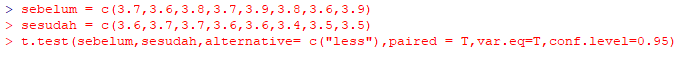
\includegraphics[width = \linewidth]{img3.png}
\end{center}
Setelah itu masukkan variabel ke dalam perintah t.test\\
\texttt{t.test(sebelum,sesudah,alternative=c("two sided"), paired=T, var.equal=T, conf.level=0.95)}
\begin{center}
    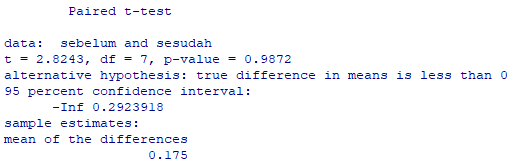
\includegraphics[width = \linewidth]{img4.png}
\end{center}
Dari output diatas diketahui bahwa $H_{0}$ diterima karena $p\_value = 0.9872 > \alpha = 0.05$

\subsection{Latihan}
\subsubsection{Latihan 1}
\paragraph{}
Sebuah perusahaan penghasil bahan bakar mobil hendak memilih satu dari dua ramuan kimia yang akan dijadikan campuran di dalam produknya. Ramuan tersebut adalah RDX dan DLL. Untuk
memutuskannya, departemen riset perusahaan tersebut mengadakan penelitian untuk menguji efisiensi penggunaan bahan bakar setelah diberi kedua campuran tersebut. Dengan memberikan 1 liter bahan
bakar untuk setiap mobil, jarak tempuh 15 mobil yang diberi bahan bakar bercampur RDX dan 15 mobil dengan bahan bakar bercampur DLL kemudian dicatat. Apakah terdapat perbedaan jarak tempuh
antara menggunakan RDX dan DLL? Data jarak tempuh (dalam kilometer) disajikan pada tabel berikut :
\begin{table}[!ht]
    \centering
\begin{tabular}{|l|l|}
\hline
RDX  & DLL  \\ \hline
5.21 & 5.29 \\ \hline
5.31 & 5.49 \\ \hline
5.32 & 5.31 \\ \hline
5.12 & 5.36 \\ \hline
5.16 & 5.47 \\ \hline
5.40 & 5.53 \\ \hline
5.29 & 5.37 \\ \hline
5.20 & 5.47 \\ \hline
5.14 & 5.48 \\ \hline
5.23 & 5.59 \\ \hline
5.22 & 5.34 \\ \hline
5.01 & 5.47 \\ \hline
5.19 & 5.53 \\ \hline
5.23 & 5.34 \\ \hline
5.40 & 5.28 \\ \hline
\end{tabular}
\end{table}
\paragraph{Jawab\\}
Dari soal di atas diketahui:
\begin{enumerate}[label = \alph*.]
    \item Hipotesis \\
        $H_{0} : \mu_{1} = \mu_{0}$ (rata-rata jarak tempuh mobil sama)\\
        $H_{1} : \mu_{1} \neq \mu_{0}$(rata-rata jarak tempuh mobil tidak sama)
    \item Tingkat signifikansi $\alpha = 5\%$
    \item Statistik uji p\_value
\end{enumerate}
Untuk menguji independen t test berdasarkan soal di atas, masukkan terlebih dahulu data dari tabel, kolom DLL dimasukkan ke dalam variabel DLL, sedangkan kolom RDX dimasukkan ke 
dalam variabel RDX.\\
Setelah itu masukkan variabel ke dalam perintah t.test\\
\texttt{t.test(RDX,DLL,alternative=c("two sided"), paired=F, var.equal=T, conf.level=0.95)}
\begin{center}
    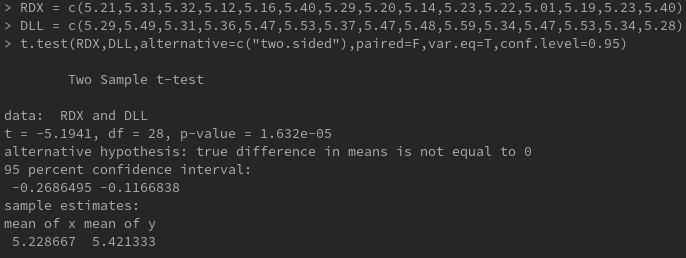
\includegraphics[width = \linewidth]{lat1.png}
\end{center}
Dari output diatas diketahui bahwa $H_{0}$ tidak diterima karena $p\_value = 0.00001632 < \alpha = 0.05$ jadi jarak tempuh mobil yang menggunakan campuran bahan bakar berbeda, berbeda pula
jarak tempuhnya.

\subsubsection{Latihan 2}
Suatu perusahaan menyatakan bahwa sejenis diet baru akan menurunkan berat badan seseorang. Berikut ini dicantumkan berat badan tujuh wanita sebelum dan sesudah mengikuti diet ini.
\begin{table}[!ht]
    \centering
\begin{tabular}{|l|l|l|}
\hline
Wanita ke- & Sesudah & Sebelum \\ \hline
1          & 58.5    & 60.0    \\ \hline
2          & 60.3    & 54.9    \\ \hline
3          & 61.7    & 58.1    \\ \hline
4          & 69.0    & 62.1    \\ \hline
5          & 64.0    & 58.5    \\ \hline
6          & 62.6    & 59.9    \\ \hline
7          & 56.0    & 54.4    \\ \hline
\end{tabular}
\end{table}
\paragraph{Jawab\\}
Dari soal di atas diketahui:
\begin{enumerate}[label = \alph*.]
    \item Hipotesis \\
        $H_{0} : \mu_{sebelum} \leq \mu_{sesudah}$ (rata-rata berat badan sebelum diet lebih kecil sama dengan)\\
        $H_{1} : \mu_{sebelum} > \mu_{sesudah}$(rata-rata berat badan sesudah diet lebih besar)
    \item Tingkat signifikansi $\alpha = 5\%$
    \item Statistik uji p\_value
\end{enumerate}
Untuk menguji dependen t test berdasarkan soal di atas, masukkan terlebih dahulu data dari tabel, kolom sesudah dimasukkan ke dalam variabel sesudah, sedangkan kolom sebelum dimasukkan ke 
dalam variabel sebelum.\\
Setelah itu masukkan variabel ke dalam perintah t.test\\
\texttt{t.test(sebelum,sesudah,alternative=c("greater"), paired=T, var.equal=T, conf.level=0.95)}
\begin{center}
    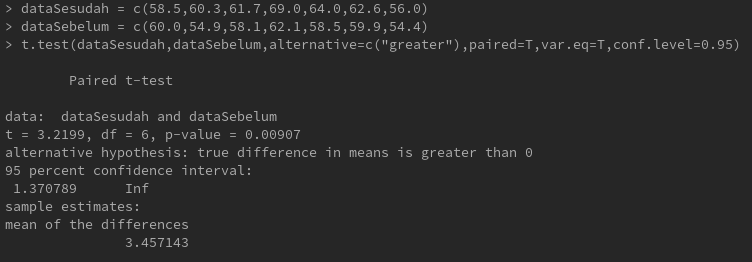
\includegraphics[width = \linewidth]{lat2.png}
\end{center}
Dari output diatas diketahui bahwa $H_{0}$ tidak diterima karena $p\_value = 0.00907 < \alpha = 0.05$ jadi berat badan wanita setelah diet lebih berat dibanding sebelum diet

\newpage

\subsection{Tugas}
\subsubsection{Tugas 1}
Untuk menghadapi persaingan dengan perusahaan roti lain, roti produksi PT. Duta Makmur yang selama ini dikemas secara sederhana akan diubah kemasannya. Untuk itu pada 15 daerah penjualan yang
berbeda, dilakukan pengamatan dengan mencatat penjualan roti dengan kemasan lama (kemasan 1), kemudian kemasan diganti dengan kemasan yang lebih atraktif (kemasan 2), dan kemudian dicatat
tingkat penjualan roti dengan kemasan yang baru pada 15 daerah yang sama. Uji apakah pengubahan kemasan membuat
rata-rata penjualan roti menjadi berbeda. Uji pada taraf keberartian 1\%
\begin{center}
    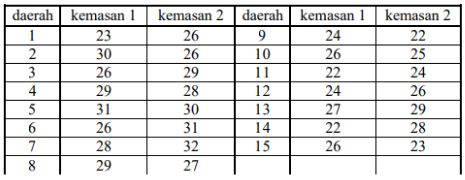
\includegraphics[scale = .6]{table.png}
\end{center}
\paragraph{Jawab\\}
Dari soal di atas diketahui:
\begin{enumerate}[label = \alph*.]
    \item Hipotesis \\
        $H_{0} : \mu_{kemasan 2} = \mu_{kemasan 1}$ (rata-rata penjualan sama)\\
        $H_{1} : \mu_{kemasan 2} \neq \mu_{kemasan 1}$(rata-rata penjualan berbeda)
    \item Tingkat signifikansi $\alpha = 1\%$
    \item Statistik uji p\_value
\end{enumerate}
Untuk menguji dependen t test berdasarkan soal di atas, masukkan terlebih dahulu data dari tabel, kolom kemasan 1 dimasukkan ke dalam variabel kemasan\_1, sedangkan kolom kemasan 2 dimasukkan
ke dalam variabel kemasan\_2.\\
Setelah itu masukkan variabel ke dalam perintah t.test\\
\texttt{t.test(kemasan\_2,kemasan\_1,alternative=c("two.sided"), paired=T, var.equal=T, conf.level=0.95)}
\begin{center}
    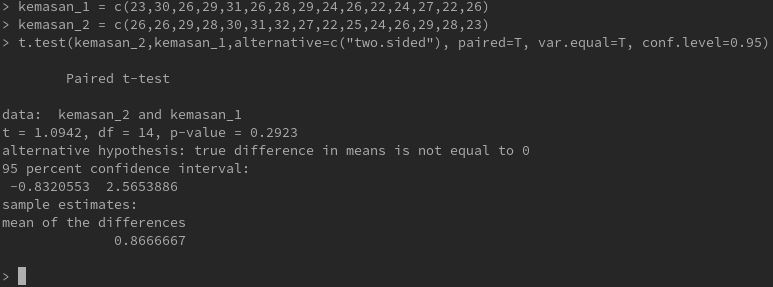
\includegraphics[width = \linewidth]{tugas1.png}
\end{center}
Dari output diatas diketahui bahwa $H_{0}$ tidak diterima karena $p\_value = 0.00907 < \alpha = 0.01$ jadi hasil penjualan kemasan 1, dan kemasan 2 berbeda.

\subsubsection{Tugas 2}
Produsen sabun ingin mengetahui apakah sabun A yang diproduksinya penjualannya lebih besar dibandingkan sabun B. Diambil sampel di 8 daerah penjualan diperoleh hasil sbb:
\begin{table}[!ht]
    \centering
\begin{tabular}{|l|l|}
\hline
Sabun A & Sabun B \\ \hline
115     & 124     \\ \hline
125     & 126     \\ \hline
132     & 122     \\ \hline
145     & 144     \\ \hline
134     & 133     \\ \hline
152     & 145     \\ \hline
155     & 160     \\ \hline
126     & 112     \\ \hline
\end{tabular}
\end{table}
\paragraph{Jawab\\}
Dari soal di atas diketahui:
\begin{enumerate}[label = \alph*.]
    \item Hipotesis \\
        $H_{0} : \mu_{A} \leq \mu_{B}$ (rata-rata penjualan sabun A tidak lebih besar dari B)\\
        $H_{1} : \mu_{A} > \mu_{B}$(rata-rata penjualan sabun A lebih besar dari B)
    \item Tingkat signifikansi $\alpha = 10\%$
    \item Statistik uji p\_value
\end{enumerate}
Untuk menguji independen t test berdasarkan soal di atas, masukkan terlebih dahulu data dari tabel, kolom sabun A dimasukkan ke dalam variabel sabun\_A, sedangkan kolom sabun B dimasukkan ke 
dalam variabel sabun\_B.\\
Setelah itu masukkan variabel ke dalam perintah t.test\\
\texttt{t.test(sabun\_B,sabun\_A,alternative=c("greater"), paired=F, var.equal=T, conf.level=0.95)}
\begin{center}
    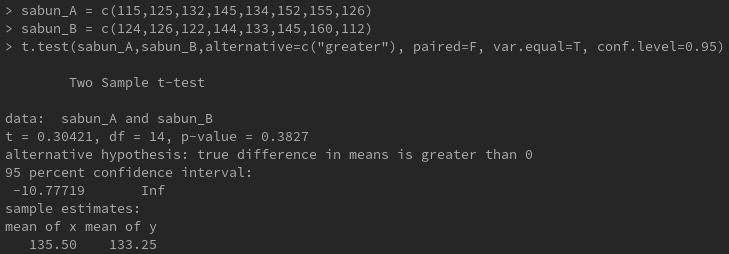
\includegraphics[width = \linewidth]{tugas2.png}
\end{center}
Dari output diatas diketahui bahwa $H_{0}$ diterima karena $p\_value = 0.3827 < \alpha = 0.10$ jadi penjualan sabun A tidak lebih besar dari B.
\end{document}
